%%%%%%%%%%%%%%%%%%%%%%%%%%%%%%%%%%%%%%%%%%%%%%%%%%%%%%%%%%%%%%%%%%%%%%
%
%         Copyright (c) 2023, gitlabci_gallery / latex
%         All rights reserved.
%
%%%%%%%%%%%%%%%%%%%%%%%%%%%%%%%%%%%%%%%%%%%%%%%%%%%%%%%%%%%%%%%%%%%%%%

\documentclass[A4,svgnames,9pt,aspectratio=169]{beamer}
%% document options:
%% - aspectratio = { 43, 169, 1610 }
%% - utf8
%%


\setlength{\footskip}{300pt}
\usepackage[french]{babel}

\hypersetup{
   allcolors   = rouge_inria,
   pdfauthor   = {Duzés Florian},
   pdftitle    = {\@title},
   pdfsubject  = {Point hebdomadaire, bi-mensuel du stage},
   pdfkeywords = {entretien, observation du travail}
}

%%%%%%%%%%%%%%%%%%%%%%%%%%%%%%%%%%%%%%%%%%%%%%%%%%%%%%%
%%
%%%%%%%%%%%%%%%%%%%%%%%%%%%%%%%%%%%%%%%%%%%%%%%%%%%%%%%

\title[titrecourt]{Réunion flash}
\subtitle{Point hebdomadaire}
\date[01/07/2025]{date long}
\author[Duzes Florian]{Duzés Florian}

\usetheme{inria}


\begin{document}

%%%%%%%%%%%%%%%%%%%%%%%%%%%%%%%%%%%%%%%%%%%%%%%%%%%%%%%
%%
%%%%%%%%%%%%%%%%%%%%%%%%%%%%%%%%%%%%%%%%%%%%%%%%%%%%%%%

\frame{\titlepage}

%%%%%%%%%%%%%%%%%%%%%%%%%%%%%%%%%%%%%%%%%%%%%%%%%%%%%%%

% Le titre des planches de sommaire est \contentsname, sa valeur
% est fixée ici à "Sommaire" par défaut.
\renewcommand{\contentsname}{Sommaire}

\frame{\tocpage}


%%--%%--%%--%%--%%--%%--%%--%%--%%--%%--%%--%%--%%--%%--%%
 
\section{État des lieux}
\frame{\sectionpage}

\begin{frame}{Point actuel}
  \begin{tikzpicture}[
    node distance=2cm,
    box/.style={rectangle, draw=black, thick, minimum width=3cm, minimum height=1cm, text centered, rounded corners, font=\bfseries},
    arrow/.style={->, >=Stealth, thick, draw=arrowColor},
    contentBoxDone/.style={rectangle, draw=black, thick, fill=board_lightGray!40, rounded corners, minimum width=3cm, minimum height=2cm, text width=3cm, align=center},
    contentBox/.style={rectangle, draw=black, thick, rounded corners, minimum width=3cm, minimum height=2cm, text width=3cm, align=center}
]

    % DESSINS
    \node[box, fill=faitColor] (fait) {Fait};
    \node[box, fill=enCoursColor, right=of fait] (en_cours) {En cours};
    \node[box, fill=aFaireColor, right=of en_cours] (a_faire) {Prévus};
    \draw[arrow] (fait) -- (en_cours);
    \draw[arrow] (en_cours) -- (a_faire);

    % Choses réalisées
    \node[contentBoxDone, below=0.5cm of fait] {
      \begin{itemize}
        \item Mise à jour de Binsec
      \end{itemize}
    };

    % En cours
    \node[contentBox, below=0.5cm of en_cours, fill=enCoursColor!15] {
        \begin{itemize}
          \item Remplir les config
          \item Gérer les dépendances
          \item Activer chaîne de compilation
          \item Compilation en x86\_64
        \end{itemize}
    };

    % Point fixer
    \node[contentBox, below=0.5cm of a_faire, fill=aFaireColor!15] {
        \begin{itemize}
            \item Chaîne de bout en bout 
            \item Couverture des architectures différentes
            \item Couverture des compilateurs
        \end{itemize}
    };
      \end{tikzpicture}

\end{frame}


%  .  .  .  .  .  .  .  .  .  .  .  .  .  .  .  .  .  .  %

\begin{frame}{Réalisation}
  \begin{tikzpicture}[
    node distance=2cm,
    box/.style={rectangle, draw=black, thick, minimum width=3cm, minimum height=1cm, text centered, rounded corners, font=\bfseries},
    arrow/.style={->, >=Stealth, thick, draw=arrowColor},
    contentBoxDone/.style={rectangle, draw=black, thick, fill=board_lightGray!40, rounded corners, minimum width=3cm, minimum height=2cm, text width=3cm, align=center},
    contentBox/.style={rectangle, draw=black, thick, rounded corners, minimum width=3cm, minimum height=2cm, text width=3cm, align=center}
]

    % DESSINS
    \node[box, fill=faitColor] (fait) {Fait};
    \node[box, fill=enCoursColor, right=of fait] (en_cours) {En cours};
    \node[box, fill=aFaireColor, right=of en_cours] (a_faire) {Prévus};
    \draw[arrow] (fait) -- (en_cours);
    \draw[arrow] (en_cours) -- (a_faire);

    % Choses réalisées
    \node[contentBoxDone, below=0.5cm of fait] {
      \begin{itemize}
        \item Gérer les dépendances
        \item Activer chaîne de compilation
        \item Compilation en x86\_64
        \item \textit{Introduction} du mémoire
      \end{itemize}
    };

    % En cours
    \node[contentBox, below=0.5cm of en_cours, fill=enCoursColor!15] {
        \begin{itemize}
          \item Remplir les config
          \item Régler les problèmes d'analyse de Binsec
          \item Chaîne de bout en bout x86\_64 
        \end{itemize}
    };

    % Point fixer
    \node[contentBox, below=0.5cm of a_faire, fill=aFaireColor!15] {
        \begin{itemize}
            \item Couverture des architectures différentes
            \item Couverture des compilateurs
        \end{itemize}
    };
      \end{tikzpicture}

\end{frame}

%%--%%--%%--%%--%%--%%--%%--%%--%%--%%--%%--%%--%%--%%--%%

\section{Une chaîne de bout en bout}
\frame{\sectionpage}

\begin{frame}{On y est}

  \begin{center}
    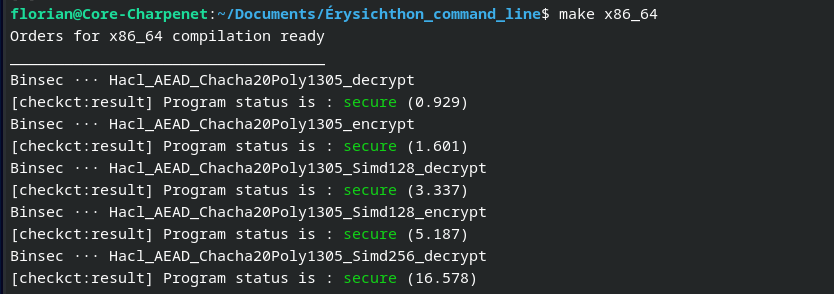
\includegraphics[trim={0 0 2cm 0},clip,scale=0.5]{imgs/reussite.png}
  \end{center}

\end{frame}

%  .  .  .  .  .  .  .  .  .  .  .  .  .  .  .  .  .  .  %

\begin{frame}{Encore des problèmes}

  \begin{block}{Les fichiers de config}
    \begin{itemize}
      \item Remplissage à 1/3
      \item Gestion des exceptions
      \item Appel aux fonctions voisines
    \end{itemize}
  \end{block}
\end{frame}

%  .  .  .  .  .  .  .  .  .  .  .  .  .  .  .  .  .  .  %

\begin{frame}{Encore des problèmes - 2}

  \begin{block}{Analyse Binsec pas automatique}
    Utilisation de "core dump"
    \begin{itemize}
      \item Affectation des variables secrètes
      \item Proposition
      \begin{enumerate}
        \item "*" -> secret
        \item liste de noms de variables
      \end{enumerate}
    \end{itemize}
  \end{block}
  \textit{Test avec analyse directement depuis code compilé ?}
\end{frame}

%  .  .  .  .  .  .  .  .  .  .  .  .  .  .  .  .  .  .  %


%%%%%%%%%%%%%%%%%%%%%%%%%%%%%%%%%%%%%%%%%%%%%%%%%%%%%%%

\section{Point avec Érysichton}
\frame{\sectionpage}

\begin{frame}{Zone de difficultés}
  \centering
  \begin{tikzpicture}[auto]

    % Styles
    \tikzstyle{startstop} = [rectangle, rounded corners, minimum width=2cm, minimum height=1cm, text centered, draw=black, fill=green!30]
    \tikzstyle{process} = [rectangle, minimum width=2cm, minimum height=1cm, text centered, draw=black, fill=orange!30]
    \tikzstyle{arrow} = [thick,->,>=stealth]
    \tikzset{zone1/.style={rectangle, rounded corners, draw=red, dashed, fill=red!10, inner sep=0.3cm}}
    \tikzset{zone2/.style={rectangle, rounded corners, draw=blue, dashed, fill=blue!10, inner sep=0.3cm}}
    \tikzset{zone22/.style={rectangle, rounded corners, draw=none, fill=blue!10, inner sep=0.3cm}}
    \tikzset{zone3/.style={rectangle, rounded corners, draw=green, dashed, fill=green!10, inner sep=0.3cm}}
    
    % Noeuds
    \node (hacl) [startstop] {Hacl*};
    \node (c) [below of=hacl] {.h};
    \node (ini) [below of=c, xshift=2cm] {.ini};
    \node (test) [below of=c, xshift=-2cm] {-test.c};
    \node (script) [below of=c] {.script};
    \node (compilateur) [process, below of=test] {Compilateur};
    \node (exe) [below of=compilateur] {-test.exe};
    \node (blanc1) [below of=script] {};
    \node (blanc2) [below of=blanc1] {};
    \node (gdb) [process, below of=blanc2] {GDB};
    \node (snap) [right of=gdb, xshift=2cm] {.snapshot};
    \node (binsec) [startstop, right of=snap, xshift=1.5cm] {Binsec};
    
    % Flèches
    \draw [arrow] (hacl) -- (c);
    \draw [red, arrow] (c) -- (ini);
    \draw [red, arrow] (c) -- (test);
    \draw [arrow] (c) -- (script);
    \draw [arrow] (test) -- (compilateur);
    \draw [arrow] (compilateur) -- (exe);
    \draw [arrow] (exe) -- (gdb);
    \draw [arrow] (script) -- (gdb);
    \draw [arrow] (gdb) -- (snap);
    \draw [arrow] (snap) -- (binsec);
    \draw [arrow] (ini) -- (binsec);

    % Zones
    % \begin{scope}[on background layer]
    %     \onslide<1>{\node [zone1, fit=(c) (ini) (test) (script)] {};}
    %     \onslide<1>{\node [zone2, fit=(script) (gdb)] {};}
    %     \onslide<1>{\node [zone2, fit=(gdb) (snap) (binsec)] {};}
    %     \onslide<1>{\draw [zone22]
    %     ([xshift=-9pt, yshift=10pt]gdb.north west) --
    %     ([xshift=9pt, yshift=10pt]gdb.north east) -- 
    %     ([xshift=1pt, yshift=-1pt]gdb.south east) -- 
    %     ([xshift=-1pt, yshift=-1pt]gdb.south west) --
    %     cycle; }
    %     \onslide<1,2>{\node [zone3, fit=(compilateur) (exe)] {};}
    % \end{scope}
    \end{tikzpicture}

\end{frame}

%  .  .  .  .  .  .  .  .  .  .  .  .  .  .  .  .  .  .  %

\begin{frame}{Utilisation de wrappeur}

  \begin{block}{Outils}
    \begin{itemize}
      \item frama-c
      \item clangml
      \item CIL
    \end{itemize}    
  \end{block}
  \pause
  En pause pour le moment - informations déjà acquise
  \begin{itemize}
    \item \textit{Optimisation future ?}
    \item Trouble avec Binsec
  \end{itemize}
  
\end{frame}

%%%%%%%%%%%%%%%%%%%%%%%%%%%%%%%%%%%%%%%%%%%%%%%%%%%%%%%

\section{Binsec patch}
\frame{\sectionpage}

\begin{frame}{Identification d'une erreur}
  \begin{block}{Problème de pile}
    \begin{itemize}
      \item Est-ce que le correctif est bon ?
      \item Compilation de binsec vers RISC-V
    \end{itemize}
  \end{block}
\end{frame}

%%%%%%%%%%%%%%%%%%%%%%%%%%%%%%%%%%%%%%%%%%%%%%%%%%%%%%%

\section{Conclusion}
\frame{\sectionpage}

\begin{frame}{Conclusion}
  \begin{block}{Objectif}
    Finir le module x86\_64.
  \end{block}

  \begin{enumerate}
    \item Remplir les configurations
    \item Générer les tests
    \item[{\makebox[0pt][l]{$\square$}\raisebox{.15ex}{\hspace{0.1em}$\checkmark$}}] \sout{Compiler les tests}
    \item[{\makebox[0pt][l]{$\square$}\raisebox{.15ex}{\hspace{0.1em}$\checkmark$}}] Analyser les tests
  \end{enumerate}
  

\end{frame}

%%%%%%%%%%%%%%%%%%%%%%%%%%%%%%%%%%%%%%%%%%%%%%%%%%%%%%%

%% Le texte est modifiable en changeant \thankyou
%% \renewcommand{\thankyou}{Thank You.}
\frame{\merci}


\end{document}

